% https://tex.stackexchange.com/questions/152952/drawing-this-diagram-in-tikz?rq=1
\documentclass[tikz,border=10pt]{standalone}
\usetikzlibrary{fit,positioning,calc}
\tikzset{decision/.style = {diamond, draw, fill=blue!20, text width=4.5em, text badly centered, node
                            distance=3cm, inner sep=0pt},
         block/.style    = {rectangle, draw, fill=black!25, text width=5em, text centered, rounded
                            corners, minimum height=4em},
         line/.style     = {draw, -latex'},
         cloud/.style    = {draw, ellipse,fill=red!20, node distance=3cm, minimum height=2em}
}
\begin{document}
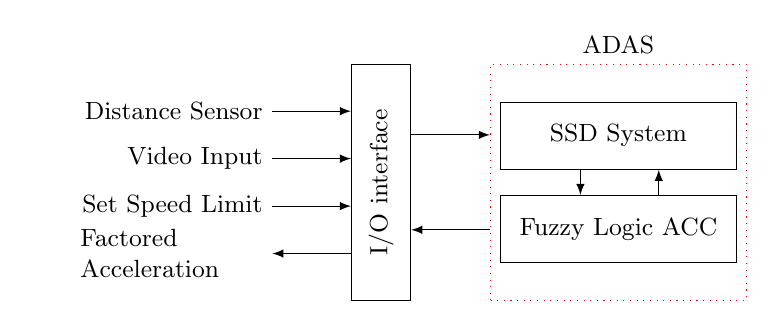
\begin{tikzpicture}[scale=2,font=\small]
    \node [draw=black,minimum width=3cm,minimum height=0.85cm] (io2) {SSD System};
    \node [draw=black,minimum width=3cm,minimum height=0.85cm, below =0.32cm of io2] (io3) {Fuzzy Logic ACC};
    \draw [latex-] ($(io2.south east)!0.33!(io2.south west)$) -- ($(io3.north east)!0.33!(io3.north west)$);
    \draw [-latex] ($(io2.south east)!0.66!(io2.south west)$) -- ($(io3.north east)!0.66!(io3.north west)$);
    \node[fit=(io2) (io3), draw=red, dotted,minimum height=3cm] (fit) {};
    \node[anchor=south] at (fit.north) {ADAS};
    \node [draw=black,rotate=90,anchor=north,minimum width=3cm,minimum height=0.75cm,left=1cm of fit,anchor=south] (io) {I/O interface};
    \draw[-latex] ($(io.south east)!0.3!(io.south west)$) -- ($(fit.north west)!0.3!(fit.south west)$);
    \draw[latex-] ($(io.south east)!0.7!(io.south west)$) -- ($(fit.north west)!0.7!(fit.south west)$);
    \foreach \x/\a in {0.2/2,0.4/4,0.6/6,0.8/8}{
    \coordinate (z\a) at ($(io.north east)!\x!(io.north west)$);
    }
    \draw[latex-](z2)--+(-.5,0) node[anchor=east]{Distance Sensor};
    \draw[latex-](z4)--+(-.5,0) node[anchor=east]{Video Input};
    \draw[latex-](z6)--+(-.5,0) node[anchor=east]{Set Speed Limit};
    \draw[-latex](z8)--+(-.5,0) node[anchor=east,minimum width=3.1cm,align=left]{Factored \\ Acceleration}; 
\end{tikzpicture}
\end{document}